%% abtex2-modelo-artigo.tex, v-1.9.7 laurocesar
%% Copyright 2012-2018 by abnTeX2 group at http://www.abntex.net.br/ 
%%
%% This work may be distributed and/or modified under the
%% conditions of the LaTeX Project Public License, either version 1.3
%% of this license or (at your option) any later version.
%% The latest version of this license is in
%%   http://www.latex-project.org/lppl.txt
%% and version 1.3 or later is part of all distributions of LaTeX
%% version 2005/12/01 or later.
%%
%% This work has the LPPL maintenance status `maintained'.
%% 
%% The Current Maintainer of this work is the abnTeX2 team, led
%% by Lauro César Araujo. Further information are available on 
%% http://www.abntex.net.br/
%%
%% This work consists of the files abntex2-modelo-artigo.tex and
%% abntex2-modelo-references.bib
%%

% ------------------------------------------------------------------------
% ------------------------------------------------------------------------
% abnTeX2: Modelo de Artigo Acadêmico em conformidade com
% ABNT NBR 6022:2018: Informação e documentação - Artigo em publicação 
% periódica científica - Apresentação
% ------------------------------------------------------------------------
% ------------------------------------------------------------------------

\documentclass[
	% -- opções da classe memoir --
	article,			% indica que é um artigo acadêmico
	11pt,				% tamanho da fonte
	oneside,			% para impressão apenas no recto. Oposto a twoside
	a4paper,			% tamanho do papel. 
	% -- opções da classe abntex2 --
	%chapter=TITLE,		% títulos de capítulos convertidos em letras maiúsculas
	%section=TITLE,		% títulos de seções convertidos em letras maiúsculas
	%subsection=TITLE,	% títulos de subseções convertidos em letras maiúsculas
	%subsubsection=TITLE % títulos de subsubseções convertidos em letras maiúsculas
	% -- opções do pacote babel --
	english,			% idioma adicional para hifenização
	brazil,				% o último idioma é o principal do documento
	sumario=tradicional
	]{abntex2}


% ---
% PACOTES
% ---

% ---
% Pacotes fundamentais 
% ---
\usepackage{lmodern}			% Usa a fonte Latin Modern
\usepackage[T1]{fontenc}		% Selecao de codigos de fonte.
\usepackage[utf8]{inputenc}		% Codificacao do documento (conversão automática dos acentos)
\usepackage{indentfirst}		% Indenta o primeiro parágrafo de cada seção.
\usepackage{nomencl} 			% Lista de simbolos
\usepackage{color}				% Controle das cores
\usepackage{graphicx}			% Inclusão de gráficos
\usepackage{microtype} 			% para melhorias de justificação
% ---
		
% ---
% Pacotes adicionais, usados apenas no âmbito do Modelo Canônico do abnteX2
% ---
\usepackage{lipsum}				% para geração de dummy text
% ---
		
% ---
% Pacotes de citações
% ---
\usepackage[brazilian,hyperpageref]{backref}	 % Paginas com as citações na bibl
\usepackage[alf]{abntex2cite}	% Citações padrão ABNT
% ---

% ---
% Configurações do pacote backref
% Usado sem a opção hyperpageref de backref
\renewcommand{\backrefpagesname}{Citado na(s) página(s):~}
% Texto padrão antes do número das páginas
\renewcommand{\backref}{}
% Define os textos da citação
\renewcommand*{\backrefalt}[4]{
	\ifcase #1 %
		Nenhuma citação no texto.%
	\or
		Citado na página #2.%
	\else
		Citado #1 vezes nas páginas #2.%
	\fi}%
% ---

% --- Informações de dados para CAPA e FOLHA DE ROSTO ---
\titulo{Comparação de defirentes aborgens para resoluções do dataset cat's vs dog's}
\tituloestrangeiro{Comparing differents approaches to solve Cat's vs Dog's dataset }

\autor{
	Lucas Mrowskovsy Paim\thanks{Programa de Pós Graduação em Inteligência Aritificial, Curitiba - PR, 80215-901; Especializando em Inteligência Artificial Aplicada pela PUCPR; Tecnólogo em Sistemas para Internet pela Universidade Positivo; E-mail: lucasmpaim1@gmail.com} 
}

\local{Brasil}
\data{2019}
% ---

% ---
% Configurações de aparência do PDF final

% alterando o aspecto da cor azul
\definecolor{blue}{RGB}{41,5,195}

% informações do PDF
\makeatletter
\hypersetup{
     	%pagebackref=true,
		pdftitle={\@title}, 
		pdfauthor={\@author},
    	pdfsubject={Modelo de artigo científico com abnTeX2},
	    pdfcreator={LaTeX with abnTeX2},
		pdfkeywords={abnt}{latex}{abntex}{abntex2}{atigo científico}, 
		colorlinks=true,       		% false: boxed links; true: colored links
    	linkcolor=blue,          	% color of internal links
    	citecolor=blue,        		% color of links to bibliography
    	filecolor=magenta,      		% color of file links
		urlcolor=blue,
		bookmarksdepth=4
}
\makeatother
% --- 

% ---
% compila o indice
% ---
\makeindex
% ---

% ---
% Altera as margens padrões
% ---
\setlrmarginsandblock{3cm}{3cm}{*}
\setulmarginsandblock{3cm}{3cm}{*}
\checkandfixthelayout
% ---

% --- 
% Espaçamentos entre linhas e parágrafos 
% --- 

% O tamanho do parágrafo é dado por:
\setlength{\parindent}{1.3cm}

% Controle do espaçamento entre um parágrafo e outro:
\setlength{\parskip}{0.2cm}  % tente também \onelineskip

% Espaçamento simples
\SingleSpacing


% ----
% Início do documento
% ----
\begin{document}

% Seleciona o idioma do documento (conforme pacotes do babel)
%\selectlanguage{english}
\selectlanguage{brazil}

% Retira espaço extra obsoleto entre as frases.
\frenchspacing 

% ----------------------------------------------------------
% ELEMENTOS PRÉ-TEXTUAIS
% ----------------------------------------------------------

%---
%
% Se desejar escrever o artigo em duas colunas, descomente a linha abaixo
% e a linha com o texto ``FIM DE ARTIGO EM DUAS COLUNAS''.
% \twocolumn[    		% INICIO DE ARTIGO EM DUAS COLUNAS
%
%---

% página de titulo principal (obrigatório)
\maketitle


% titulo em outro idioma (opcional)



% resumo em português
\begin{resumoumacoluna}
 Este trabalho tem por objetivo comparar diferentes técnicas para a solução do dataset cat's vs dogs, a versão utilizada por este trabalho é uma base fornecida pelo Tensorflow com cerca de três mil imagens de gatos e cachorros para realizar a classificação de imagens, foram utilizadas as técnicas transfer learning utilizando modelo shallow e fine tuning e também criado uma rede neural densa a partir do zero. Todos os modelos tiveram resultados satisfatórios para o problema proposto.
 
 \vspace{\onelineskip}
 
 \noindent
 \textbf{Palavras-chave}: deep-learning. tensorflow. cnn. cats vs dogs.
\end{resumoumacoluna}


% resumo em inglês
\renewcommand{\resumoname}{Abstract}
\begin{resumoumacoluna}
 \begin{otherlanguage*}{english}

This work aims to compare different techniques for the solution of the cat's vs dogs dataset, the version used by this work is a base provided by Tensorflow with about three thousand images of cats and dogs to perform the image classification, were used transfer learning techniques using shallow and fine tuning models and also created a dense neural network from scratch. All models had satisfactory results for the proposed problem.

   \vspace{\onelineskip}
 
   \noindent
   \textbf{Keywords}: deep-learning. tensorflow. cnn. cats vs dogs.
 \end{otherlanguage*}  
\end{resumoumacoluna}

% ]  				% FIM DE ARTIGO EM DUAS COLUNAS
% ---

% ----------------------------------------------------------
% ELEMENTOS TEXTUAIS
% ----------------------------------------------------------
\textual

% ----------------------------------------------------------
% Introdução
% ----------------------------------------------------------
\section{Introdução}

Segundo \citeonline{handsOnML}, apesar de os computadores já terem conseguido feitos notáveis como vencer o campeão mundial de xadrez em 1996, eles ainda não conseguiam realizar tarefas triviais, como detectar um animal em uma foto, o que para nós humanos é algo extremamente trivial, isto ainda segundo \citeonline{handsOnML} é devido ao nosso cérebro enviar para nosso subconsciente apenas informações de auto-nível, as redes neurais convolucionais (CNN), surgiram do estudo de nosso córtex visual e essas redes tem sido utilizadas como o principal meio para detecção de imagens desde então.

Neste trabalho será abordado algumas diferentes técnicas para a resolução do dataset cats vs dogs já pré-processada disponibilizada pelo Google na página do Tensorflow, onde foram removidas cerca de 1738 imagens corrompidas. 

% ----------------------------------------------------------
% Seção de explicações
% ----------------------------------------------------------
\section{Método}

O dataset utilizado por este trabalho, foi a "cats vs dogs" disponibilizada pelo Google em sua página da tensorflow, esta base contém 3 mil imagens de gatos e cachorros e seu propósito é ensinar a computadores a classificar fotos destes dois animais.
A base está dividida em treinamento e validação, onde respectivamente temos, 2 mil imagens para treinamento e mil imagens para validação, ou seja, aproximadamente 30\% da base voltada para validação.

As técnicas utilizadas para este trabalho são:

 \begin{description}
	\item[Transfer-learning baseada em extrator de caracterísicas] é utilizada uma rede previamente treinada como extrator de caracterísicas, e estas são utilizadas para treinar modelos razos, como: SVM, KNN, etc.
	\item[Transfer-learning baseado em fine-tuning] é utilizada uma rede previamente treinada, em que as camadas convolucionais do modelo são congeladas, e as camadas densas são retreinadas para o novo problema.
	\item[From scratch] Criar e treinar um modelo a partir de um novo projeto, ou seja, sem reuilizar redes previamente treinadas.
\end{description}


\subsection{Transfer Learning Shallow}

O modelo pré-treinado utilizado por este trabalho é a Xception que é uma rede treinada utilizando a base \citeonline{imagenet}, que é uma base de com milhares de imagens utilizada e alimentada pela comunidade cientifica.

Foram extraídos as características em arquivos CSV, esta extração resultou em 2048 características para cada uma das imagens, o dataframe de treinamento obteve o seguinte shape:

\begin{verbatim}
	(2000, 2048)
\end{verbatim}

Utilizando a técnica t-SNE, que segundo \citeonline{t-SNE}, é uma técnica de redução de dimensionalidade estocástica, ou seja, utilizando está técnica é possível reduzir um vetor de tamanho \(N\) para um de tamanho \(X\), onde \(X < N\), foi realizada a redução das bases de características e apresentadas gráficamente, para assim analisar o quão bem distribuídos estão as classes, estes gráficos podem ser conferinos na \autoref{tsne-train-transfer-shallow} e \autoref{tsne-val-transfer-shallow}

É possível notar estas características conseguem separar quase que perfeitamente as duas classes (gatos e cães), já na visão reduzida que temos na plotagem do t-SNE, com isso não é necessário um modelo muito robusto para que se obtenha resultados satisfatórios. 

O modelo shallow escolhido para este trabalho é o Naive Bayes.

Segundo, \citeonline{naive-bayes-britto}, o teorema de Bayes consiste em uma abordagem probabilística para aprendizagem, calculando assim a probabilidade de uma característica \(X\) de um vetor de prever determinada classe.

A técnica de Naive Bayes, assume que todas as caractéristicas no vetor são independentes, por isso, é chamado de Naive (do inglês Ingênuo), pois determinadas caracterísicas podem estar relacionadas entre si, o que faz com que essa técnica tenha um resultado inferior a ténica de Redes Bayesianas que consideram que os atributos podem ou não ser relacionados, isto é, a característica \(X\) pode ou não estar diretamente relacionada a característica \(Y\).

\subsubsection{Resultados do Treinamento}

Como esperado, o resultado foi extremamente satisfatório, conseguindo até 97,6\% de acurácia.


\begin{verbatim}
	Acurácia Naive Bayes Validação: 0.976
\end{verbatim}

A matrix de confusão pode ser consultada na: \autoref{cm-naive-bayes}.
\subsection{Transfer Learning - Fine Tunning}


\subsubsection{Resultados do Treinamento}
\subsection{Model from Scratch}

O modelo criado do zero, foi montado baseado no modelo proposto pelo \citeonline{tensorflow-cats-vs-dogs} e em algumas configurações da Xception, sua arquitetura proposta foi:


\begin{verbatim}
_________________________________________________________________
Layer (type)                 Output Shape              Param #   
=================================================================
conv2d_3 (Conv2D)            (None, 299, 299, 16)      448       
_________________________________________________________________
max_pooling2d_3 (MaxPooling2 (None, 149, 149, 16)      0         
_________________________________________________________________
conv2d_4 (Conv2D)            (None, 149, 149, 32)      4640      
_________________________________________________________________
max_pooling2d_4 (MaxPooling2 (None, 74, 74, 32)        0         
_________________________________________________________________
conv2d_5 (Conv2D)            (None, 74, 74, 64)        18496     
_________________________________________________________________
max_pooling2d_5 (MaxPooling2 (None, 37, 37, 64)        0         
_________________________________________________________________
flatten_1 (Flatten)          (None, 87616)             0         
_________________________________________________________________
dropout_1 (Dropout)          (None, 87616)             0         
_________________________________________________________________
dense_2 (Dense)              (None, 512)               44859904  
_________________________________________________________________
dense_3 (Dense)              (None, 1)                 513       
=================================================================
Total params: 44,884,001
Trainable params: 44,884,001
Non-trainable params: 0
_________________________________________________________________
\end{verbatim}

\subsubsection{Resultados do Treinamento}

O resultado preliminar foi de 85,1\% de acurácia na base de teste e 68.8\% na base de validação.


\begin{verbatim}
loss: 0.3271 - accuracy: 0.8510 - val_loss: 0.6158 - val_accuracy: 0.6886
\end{verbatim}


É um resultado decepcionante considerando que um modelo shallow consiguiu 97\% de acurácia, porém, não foram aplicados meios de se melhorar esta rede para esta quantidade de imagens, que seria aplicar técnicas de aumento de dados, ou seja, aplicar transformações na imagem para que cada imagem gere N outras imagens, o que ajuda no treinamento da rede.

A matrix de confusão pode ser consultada na: \autoref{cm-from-scratch}, 

% ----------------------------------------------------------
% ELEMENTOS PÓS-TEXTUAIS
% ----------------------------------------------------------
\postextual

% ----------------------------------------------------------
% Referências bibliográficas
% ----------------------------------------------------------
\bibliography{references}

% ----------------------------------------------------------
% Glossário
% ----------------------------------------------------------
%
% Há diversas soluções prontas para glossário em LaTeX. 
% Consulte o manual do abnTeX2 para obter sugestões.
%
%\glossary

% ----------------------------------------------------------
% Apêndices
% ----------------------------------------------------------


% ----------------------------------------------------------
% Anexos
% ----------------------------------------------------------
\cftinserthook{toc}{AAA}
% ---
% Inicia os anexos
% ---
%\anexos

\begin{anexosenv}


\begin{figure}[htb]
	\caption{\label{tsne-train-transfer-shallow}TSNE - Treinamento - TransferLearning Shallow}
	\begin{center}
		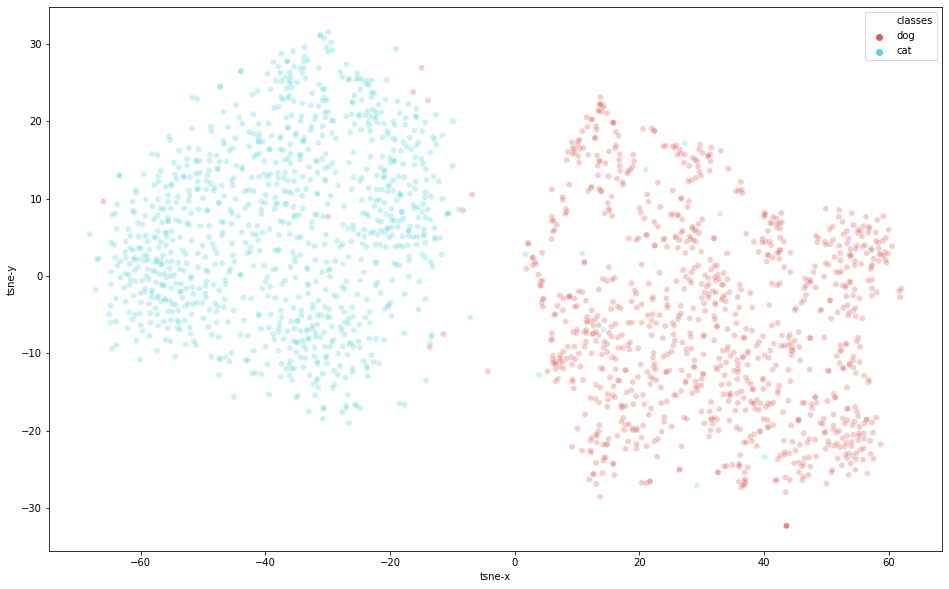
\includegraphics[scale=0.5]{images/train_dataset_view.png}
	\end{center}
	\legend{Fonte: O Autor}
\end{figure}

\begin{figure}[htb]
	\caption{\label{tsne-val-transfer-shallow}TSNE - Validação - TransferLearning Shallow}
	\begin{center}
		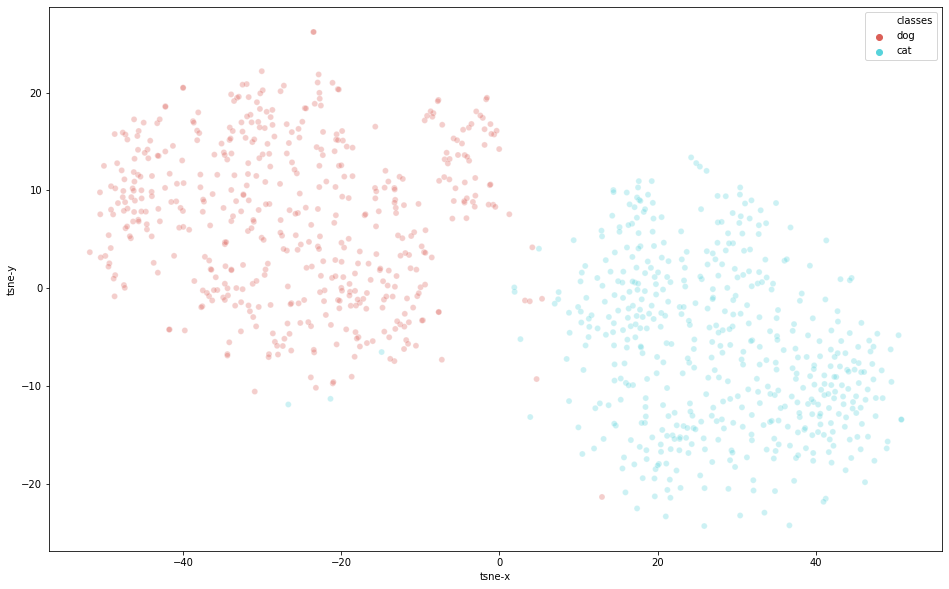
\includegraphics[scale=0.5]{images/val_dataset_view.png}
	\end{center}
	\legend{Fonte: O Autor}
\end{figure}

\begin{figure}[htb]
	\caption{\label{cm-naive-bayes} Matrix de confusão - Naive Bayes - Normalizada}
	\begin{center}
		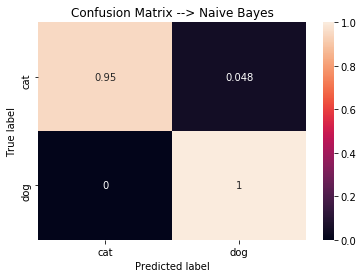
\includegraphics[scale=0.5]{images/confusion_matrix_naive_bayes.png}
	\end{center}
	\legend{Fonte: O Autor}
\end{figure}

\end{anexosenv}


\end{document}
